% Describe the problem you set out to solve and the extent of
% your success in solving it. You should include the aims and
% objectives of the project in order of importance and try to
% outline key aspects of your project for the reader to look for
% in the rest of your report.

When the Rubik's Cube was globally released in 1980, it became an instant success, selling around 200 million units by the end of 1983 \cite{unitssold}. The Rubik's Cube also quickly became a popular subject of research for computer scientists, in part due to the massive 43 quintillion possible states \cite{states} that the cube can be in. Many different algorithms were designed to try and solve the cube in as few a number of moves as possible, but it wasn't until 1997 that Richard E. Korf published a paper \cite{korf} describing a method to solve the Rubik's Cube optimally (the shortest possible number of moves to solve any given cube state) by using large lookup tables called pattern databases\cite{patterndatabases} as a heuristic function to guide an IDA* search algorithm. 

% god number stuff here

The widespread success of the Rubik's Cube also led to the creation of a number of different variants of the puzzle, each working similarly to the Rubik's Cube but of different shapes and sizes. The Kilominx is one of these variants, part of the larger "minx" family of dodecahedron-shaped puzzles. The Kilominx is a 2x2 dodecahedral puzzle with 12 faces and 20 cubies (the individual cube-shaped elements of the puzzle). Although some research has been done on tightening the bounds of its God's Number, no optimal solver has previously been created for the puzzle.

\begin{figure}[h]
    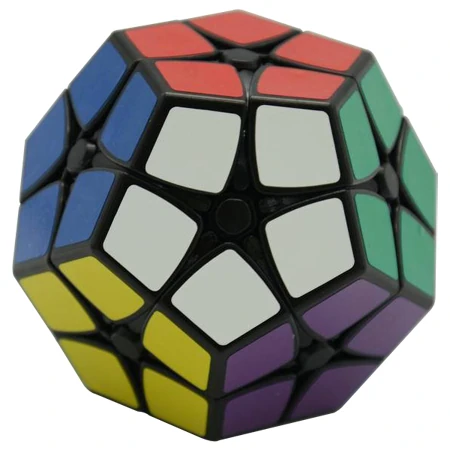
\includegraphics[width=0.4\textwidth]{kilominx}
    \centering
    \caption{An image of a Kilominx.}
    % Image URL: https://static.wikia.nocookie.net/speedcubesolving/images/8/88/4941_P_1467693201156-1-.jpg/revision/latest?cb=20180218173628
    % Website URL: https://speedcubesolving.fandom.com/wiki/Kilominx
\end{figure}

\section{Objectives}